% Ubah judul dan label berikut sesuai dengan yang diinginkan.
\section{Desain dan Implementasi}
\label{sec:desaindanimplementasi}

Pada penelitian ini, diintegrasikan teknologi visi komputer dengan sistem tertanam agar dapat mengontrol gerak kursi roda menggunakan gerakan mata (\emph{eye gesture}). Sistem dibuat menggunakan \emph{framework} MediaPipe Facemesh. Berikut merupakan blok diagram sistem yang diimplementasikan dalam penelitian ini:

%Gambar 3.1
\begin{figure} [ht] \centering
  % Nama dari file gambar yang diinputkan
  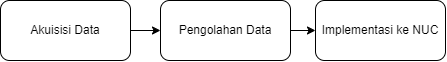
\includegraphics[scale=0.55]{gambar/paper1.png}
  % Keterangan gambar yang diinputkan
  \caption{Blok Diagram Sistem}
  % Label referensi dari gambar yang diinputkan
  \label{fig:sistem}
\end{figure}

\subsection{Akuisisi Data}

Dalam mengerjakan penelitian ini, langkah pertama yang dilakukan adalah pengambilan citra menggunakan kamera atau sumber gambar lainnya. Citra yang diambil harus cukup jelas dan terfokus pada area wajah agar fitur mata dapat diidentifikasi dengan akurat. Tahapan akuisisi data dapat dilihat pada Gambar \ref{fig:akuisisi}.

%Gambar 3.1
\begin{figure} [ht] \centering
  % Nama dari file gambar yang diinputkan
  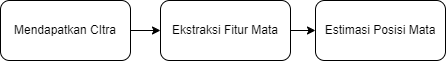
\includegraphics[scale=0.55]{gambar/paper2.png}
  % Keterangan gambar yang diinputkan
  \caption{Blok Diagram Akuisisi Data}
  % Label referensi dari gambar yang diinputkan
  \label{fig:akuisisi}
\end{figure}

Ekstrasi fitur mata adalah proses yang melibatkan penggunaan bahasa pemrograman Python, \emph{library} OpenCV, dan \emph{framework} MediaPipe. Dalam konteks ini, Mediapipe berperan penting dalam memperoleh informasi titik \emph{landmark} yang signifikan terhadap objek yang diidentifikasi. \emph{Landmarks} inilah yang menjadi dasar pembentukan representasi visual dari pose tersebut.

Pengenalan pose adalah proses yang melibatkan penggunaan bahasa pemrograman Python, \emph{library} OpenCV, dan \emph{framework} MediaPipe. Dalam konteks ini, Mediapipe berperan penting dalam memperoleh informasi titik \emph{landmark} yang signifikan terhadap objek yang diidentifikasi. \emph{Landmarks} inilah yang menjadi dasar pembentukan representasi visual dari pose tersebut.

Proses estimasi posisi mata dilakukan dengan mendeteksi keberadaan mata pada citra yang didapatkan. Setelah posisi mata didapatkan, selanjutnya dilakukan deteksi untuk 40 titik landmark pada bagian kelopak mata dan iris mata. Untuk melakukan estimasi posisi mata, beberapa titik \emph{landmark} akan digambarkan dan diwarnai dengan warna yang unik untuk membantu membedakan setiap bagian mata seperti yang dapat dilihat pada Gambar \ref{fig:estimasi}.

%Gambar 3.1
\begin{figure} [ht] \centering
  % Nama dari file gambar yang diinputkan
  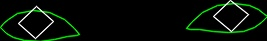
\includegraphics[scale=0.55]{gambar/bab4/30.jpg}
  % Keterangan gambar yang diinputkan
  \caption{Estimasi Posisi Mata menggunakan MediaPipe}
  % Label referensi dari gambar yang diinputkan
  \label{fig:estimasi}
\end{figure}

\subsection{Pengolahan Data}

Setelah proses estimasi posisi mata selesai, maka langkah selanjutnya ada mengelompokkan citra-citra hasil estimasi ke dalam dataset. Dataset ini akan memiliki 3 kelas berbeda, mewakili perintah untuk bergerak ke kanan, bergerak ke kiri, dan berhenti. Kelas ini mewakili perintah dasar untuk menggerakkan kursi roda. 

Untuk meningkatkan performa dan akurasi, maka dataset melewati proses optimasi menggunakan algoritma \emph{Convolutional Neural Network} (CNN). Langkah ini melibatkan penyesuaian dan peningkatan model CNN untuk meningkatkan akurasi dan efisiensi dalam deteksi mata. Untuk model CNN yang dipakai pada penelitian ini dapat dilihat pada Gambar \ref{fig:3dlayer}.

%Gambar 3.1
\begin{figure} [ht] \centering
  % Nama dari file gambar yang diinputkan
  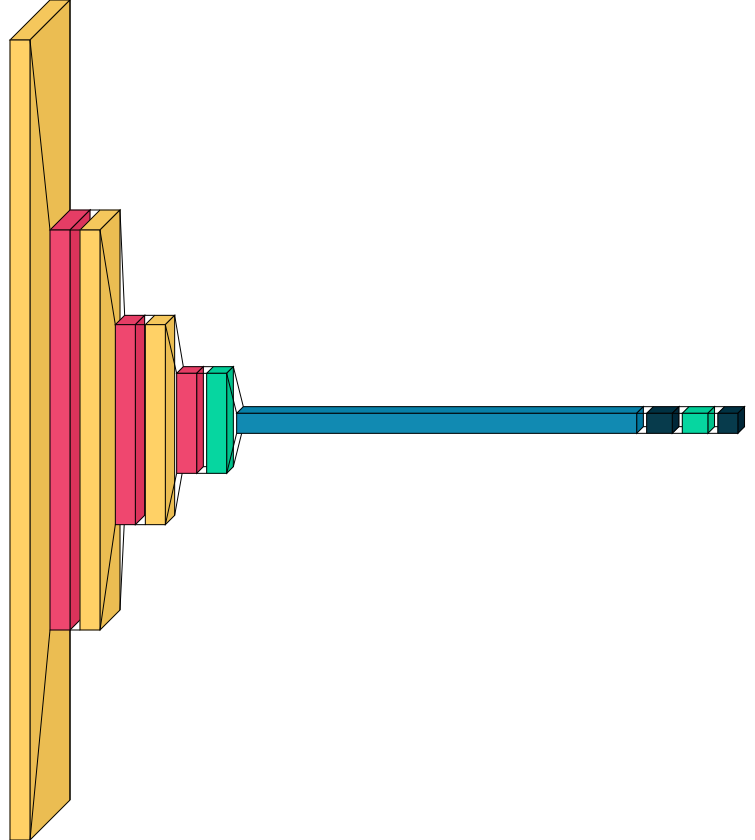
\includegraphics[scale=0.2]{gambar/bab3/3dlayer.png}
  % Keterangan gambar yang diinputkan
  \caption{Layer CNN 3 Dimensi}
  % Label referensi dari gambar yang diinputkan
  \label{fig:3dlayer}
\end{figure}

Sebelum dataset di-\emph{training} menggunakan \emph{layer} CNN, dilakukan beberapa teknik \emph{preprocessing} seperti augmentasi data dan \emph{tuning} parameter. Augmentasi data dilakukan untuk meningkatkan variasi data pelatihan dan mencegah \emph{overfitting}. Teknik augmentasi yang digunakan antara lain \emph{rotation, shearing}, dan \emph{brightness}. Selain augmentasi, \emph{tuning} parameter juga merupakan bagian penting dalam proses ini. \emph{Tuning} parameter melibatkan pengaturan \emph{hyperparameter} model seperti jumlah lapisan konvolusi, ukuran filter, ukuran kernel pooling, tingkat \emph{dropout}, dan ukuran \emph{batch}. Ditambahkan juga beberapa \emph{callbacks} yaitu \emph{rlrop} dan \emph{early stop}. Proses ini bertujuan untuk menemukan kombinasi parameter yang optimal sehingga model dapat dilatih secara efisien dan akurat.

\subsection{Implementasi ke NUC}

Implementasi sistem deteksi gerakan mata ke Intel NUC dimulai dengan menginstal pustaka perangkat lunak yang diperlukan, seperti Python, OpenCV, dan Mediapipe, ke dalam perangkat tersebut. Model yang telah dilatih kemudian diintegrasikan dengan program kontrol kursi roda, menghubungkan input dari kamera ke sinyal keluaran untuk motor kursi roda. Intel NUC terhubung ke kamera melalui port USB dan berkomunikasi dengan motor kursi roda melalui protokol serial. Sistem ini dioptimalkan untuk mencapai keseimbangan antara kecepatan dan akurasi, dengan pengaturan parameter model dan komunikasi sehingga memungkinkan kendali kursi roda berbasis gerakan mata yang akurat dan responsif.